\documentclass{beamer}

\newenvironment{tightcenter}{%
  \setlength\topsep{0pt}
  \setlength\parskip{0pt}
  \begin{center}
}{%
  \end{center}
}

\mode<presentation>
{
  \usetheme{Copenhagen}
  %%\usecolortheme[RGB={173,222,25}]{structure}
  \usecolortheme[RGB={46,3,140}]{structure}
  \setbeamertemplate{items}[circle]
  \setbeamercovered{transparent}
}

\usepackage[polish]{babel}
\usepackage{chessfss}
\usepackage{hyperref}
\usepackage{qtree}
\usepackage{mathtools}
\usepackage{dirtytalk}
\usepackage{epigraph}
\usepackage{textgreek}
\usepackage[utf8]{inputenc}
\usepackage{times}
\usepackage[T1]{fontenc}
\usepackage{tikz}
\usepackage{csquotes}
\usepackage{amsmath}
\usepackage{fancyvrb}
\usepackage{ulem}
\usepackage{adjustbox}

\newenvironment{Snippet}{\Verbatim[samepage=true]}{\endVerbatim}

\title{\textbf{Czego o architekturze nauczyła mnie praca nad własnym edytorem kodu}}

\author{Panicz Maciej Godek}

\institute{
  \tiny{\href{mailto:godek.maciek@gmail.com}{\textbf{godek.maciek@gmail.com}}} 
}

\date{\textbf{4developers Gdańsk}, 26.09.2023}

\begin{document}

\begin{frame}
  \titlepage
\end{frame}

\begin{frame}{Architektura?}
  \begin{center}
    
\includegraphics[height=0.7\paperheight]{jenzyk.png}
    \end{center}
\end{frame}

\begin{frame}{Plan prezentacji:}
  \begin{itemize}\pause
  \item wizje i inspiracje\pause
  \item 3 dema\pause
  \item design/bebechy
  \end{itemize}
\end{frame}

\begin{frame}{Składnia Lispa}
  \begin{tabular}{ l r }
    \textbf{JavaScript} & \textbf{Lisp/Scheme} \\ \pause
    \texttt{f(X, Y)} & \texttt{(f X Y)} \\ \pause
    \texttt{2 + 2} & \texttt{(+ 2 2)} \\ \pause
    \texttt{2 + 3 * 4} & \texttt{(+ 2 (* 3 4))} \\ \pause
    \texttt{function f(X, Y) \{ ... \}} & \texttt{(define (f X Y) ...)} \\ \pause
    \texttt{?} & \texttt{'(+ 2 2)} \\ \pause
    \texttt{?} & \texttt{(quote (+ 2 2))} \\ \pause
    \texttt{?} & \texttt{\#;(+ 2 2)}
  \end{tabular}
\end{frame}

\begin{frame}{Semantyka Lispa}
  \texttt{(car '(+ 2 2)) ===> +} \\ \pause
  \texttt{(cdr '(+ 2 2)) ===> (2 2)} \\ \pause
  \texttt{(cons '* '(2 2)) ===> (* 2 2)} \\ \pause
  \texttt{(cons 'a 'b) ===> (a .\ b)} \\ \pause
  \texttt{(cons 'a '()) ===> (a .\ ()) === (a)}
\end{frame}

\begin{frame}{Emacs}
  \begin{center}
    
\includegraphics[height=0.7\paperheight]{emacs.png}
  \end{center}
\end{frame}

\begin{frame}{Dema}
  \begin{center}
    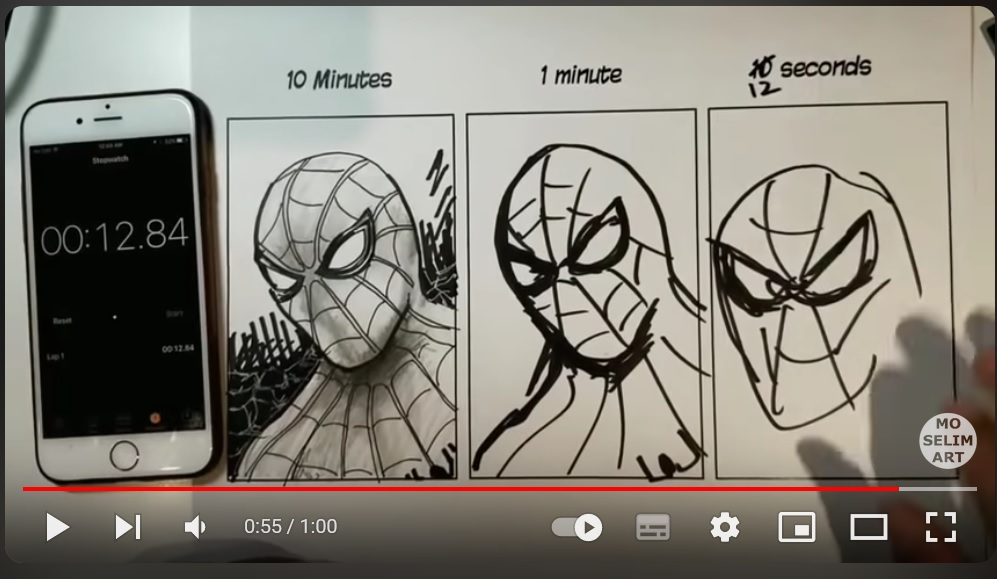
\includegraphics[height=0.7\paperheight]{drawing-spiderman.jpg}
  \end{center}
\end{frame}

\begin{frame}{Zagadnienia}
  \begin{itemize}\pause
  \item domieszki\pause
  \item interfejsy\pause
  \item jak pisać dobre ``testy''\pause
  \item architektura 3 front-endów\pause
  \item reprezentacja dokumentu - właściwości\pause
  \item parametry\pause
  \item kontynuacje i konstrukcje sterujące
  \end{itemize}
\end{frame}

\end{document}
